\chapter{Appendix}
%\section{Morphologischer Kasten}
%\label{sec:Anhang_1}


\begin{figure}[H]
\centering
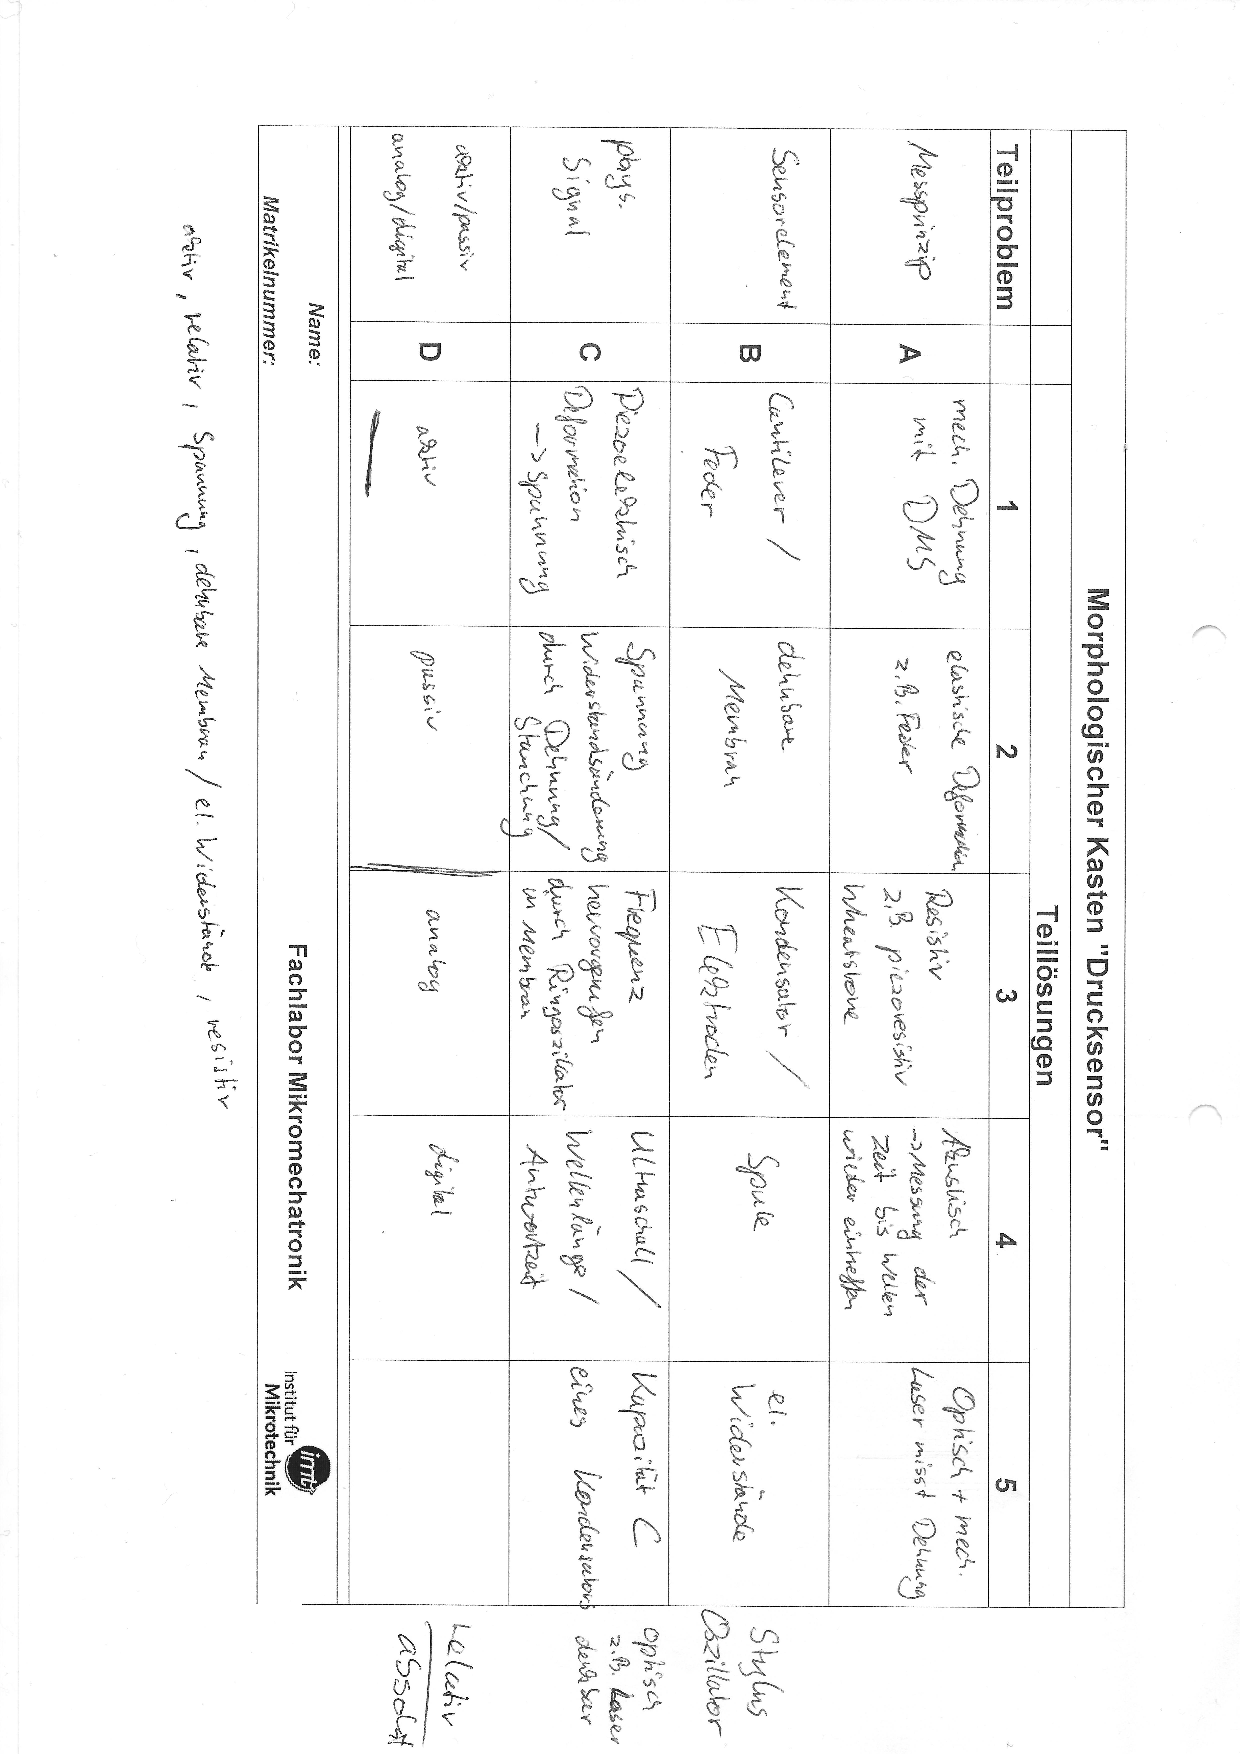
\includepdf[pages={1}, scale=0.7]{figures/Scan1.pdf}
\end{figure}

\newpage
\begin{figure}[H]
	\centering
	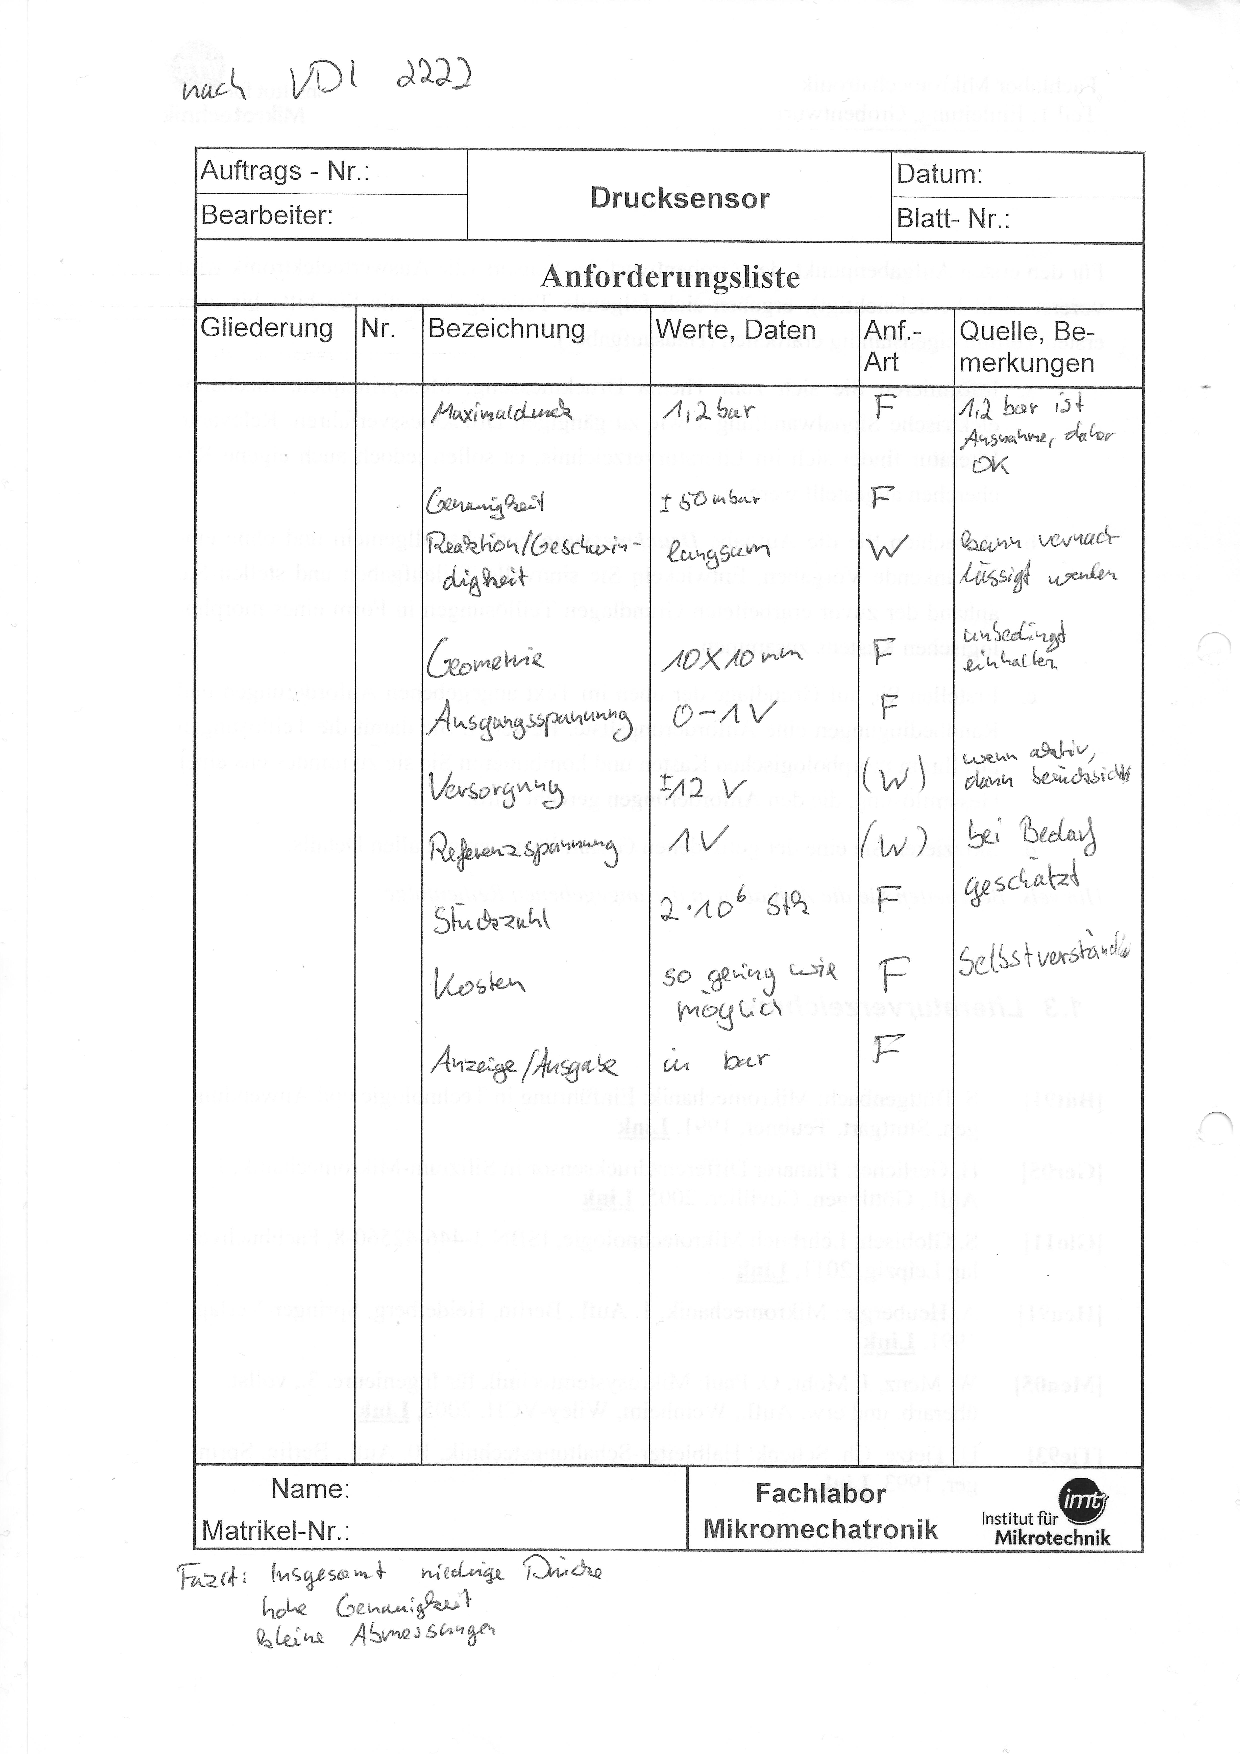
\includepdf[pages={1}, scale=0.7]{figures/Scan2.pdf}
\end{figure}

\newpage

%\section{Anforderungsliste}
%\label{sec:Anhang_2}
\begin{figure}[H]
	\centering
	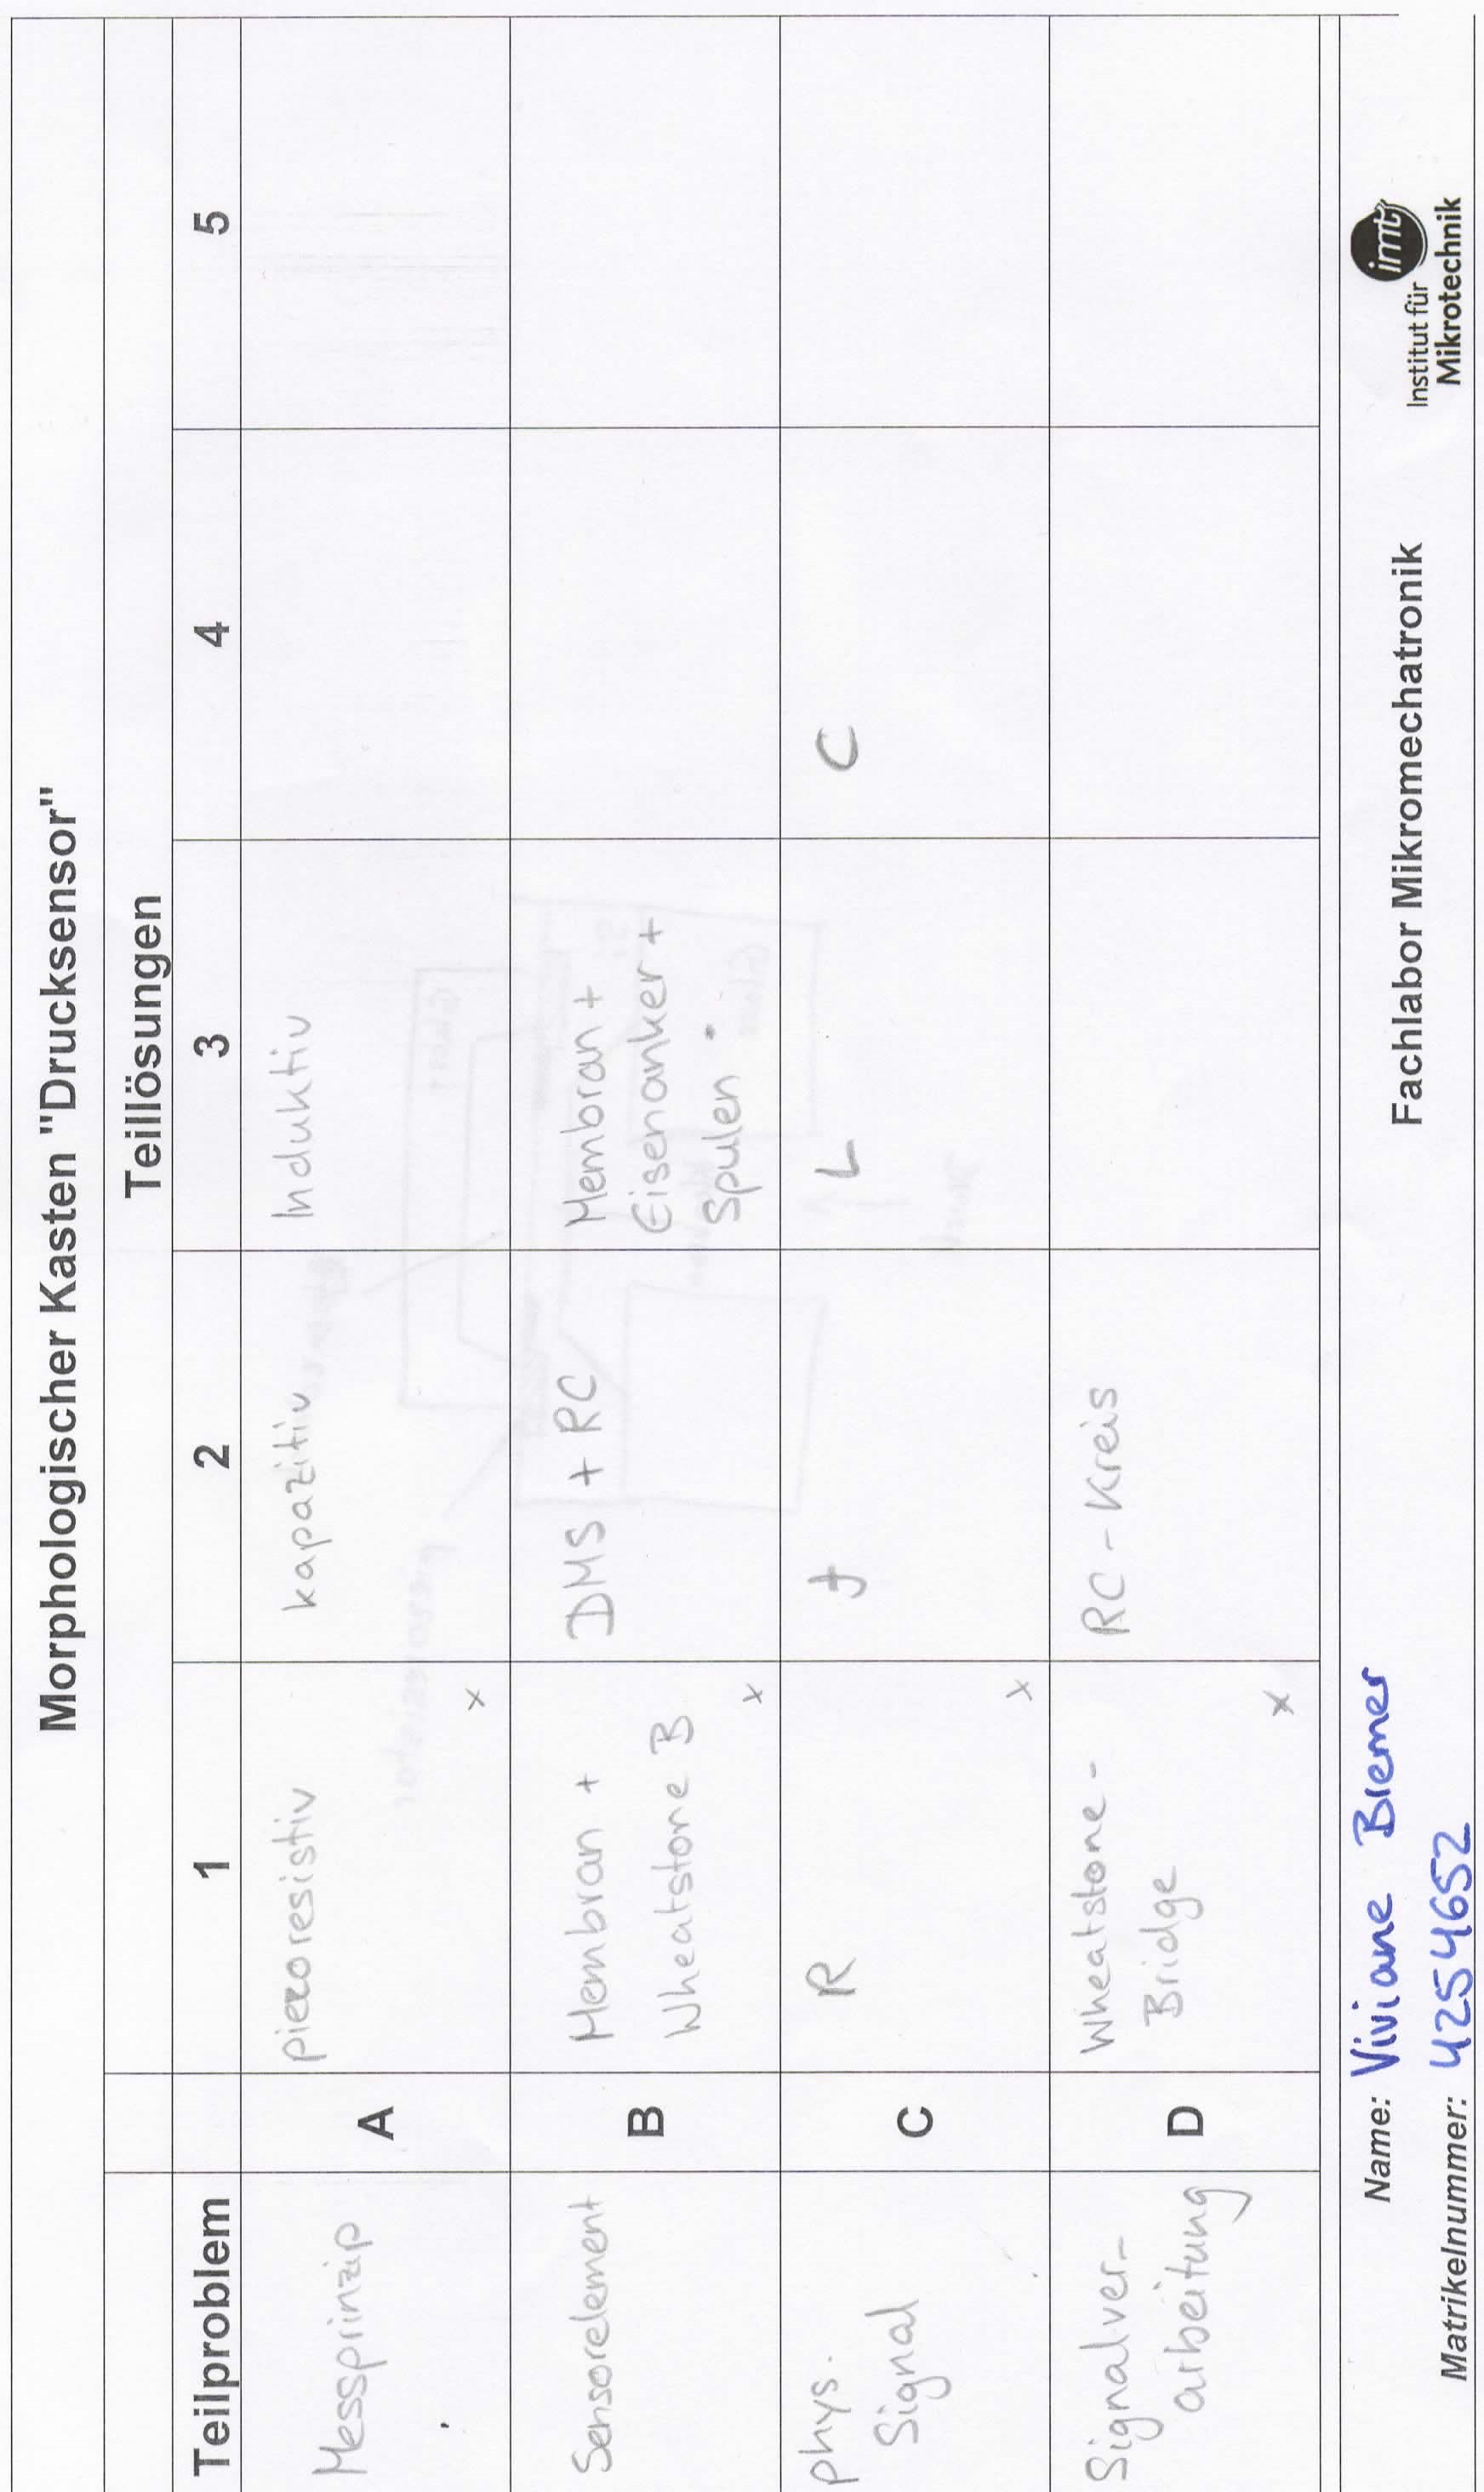
\includegraphics[width=0.7\textwidth]{figures/MorphologischerKasten_Bremer.png}
\end{figure}

\newpage

\begin{figure}[H]
	\centering
	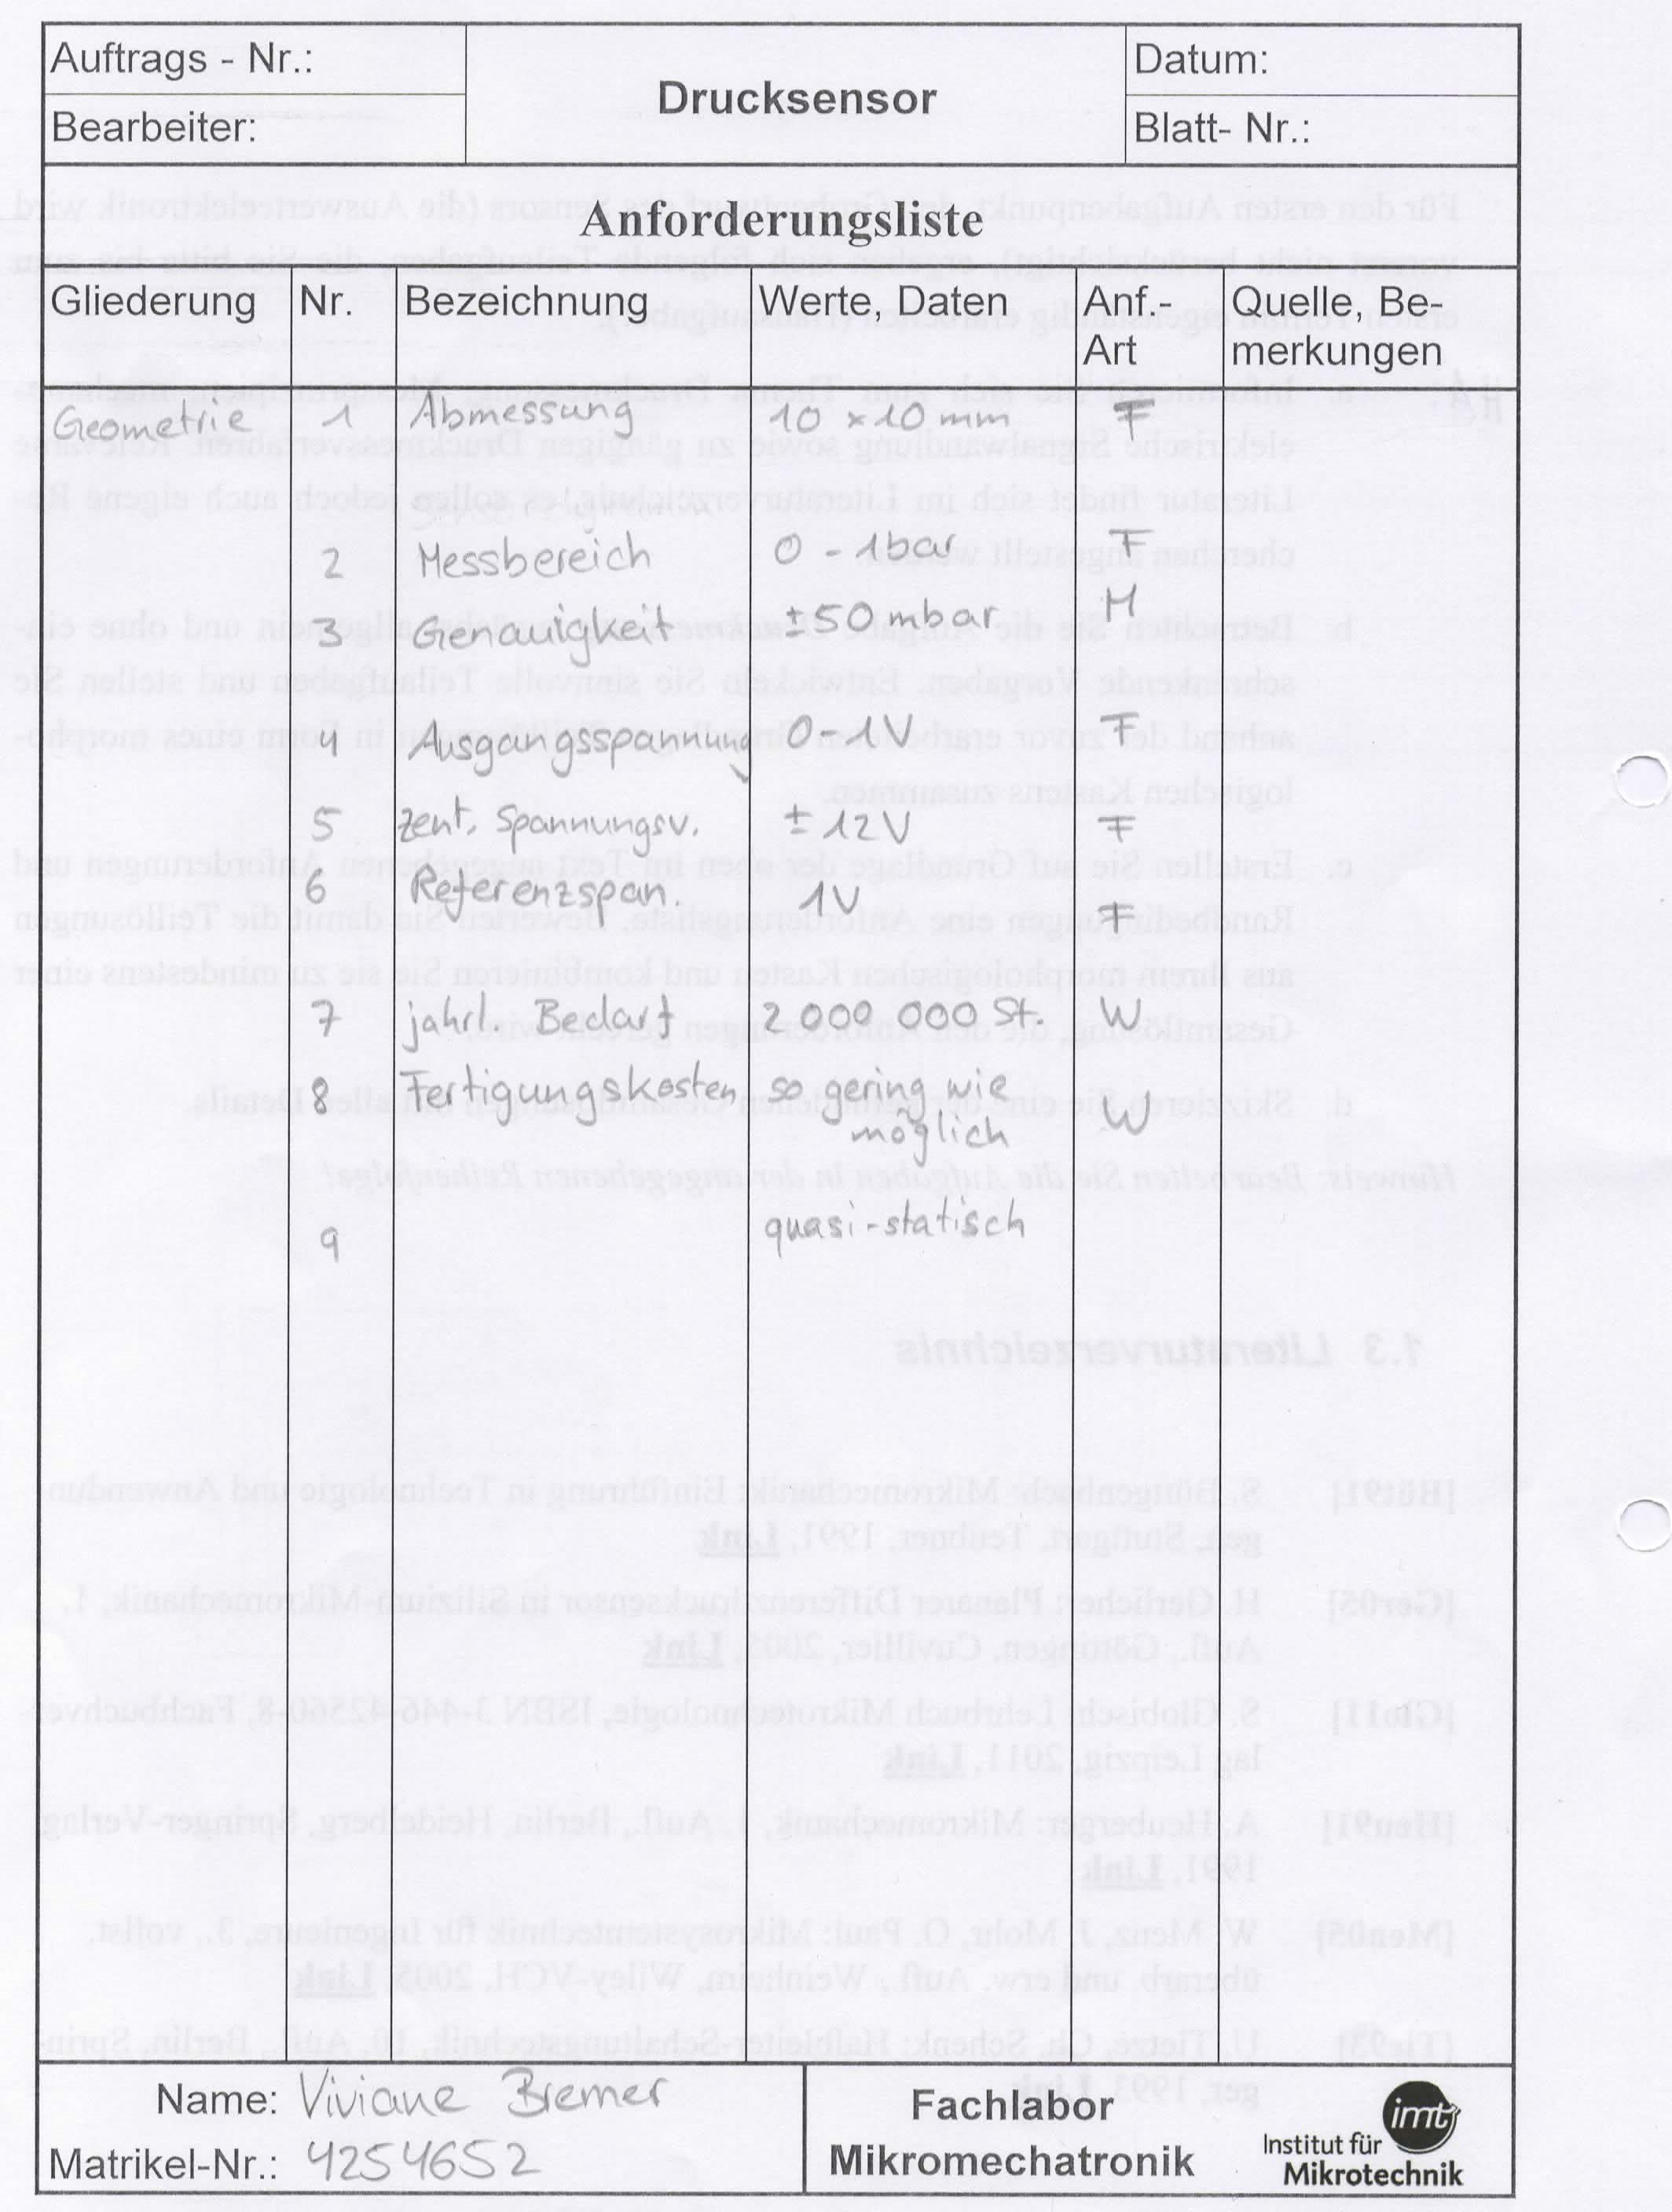
\includegraphics[width=0.9\textwidth]{figures/Anforderungsliste_Bremer.png}
\end{figure}

\newpage

\begin{figure}[H]
	\centering
	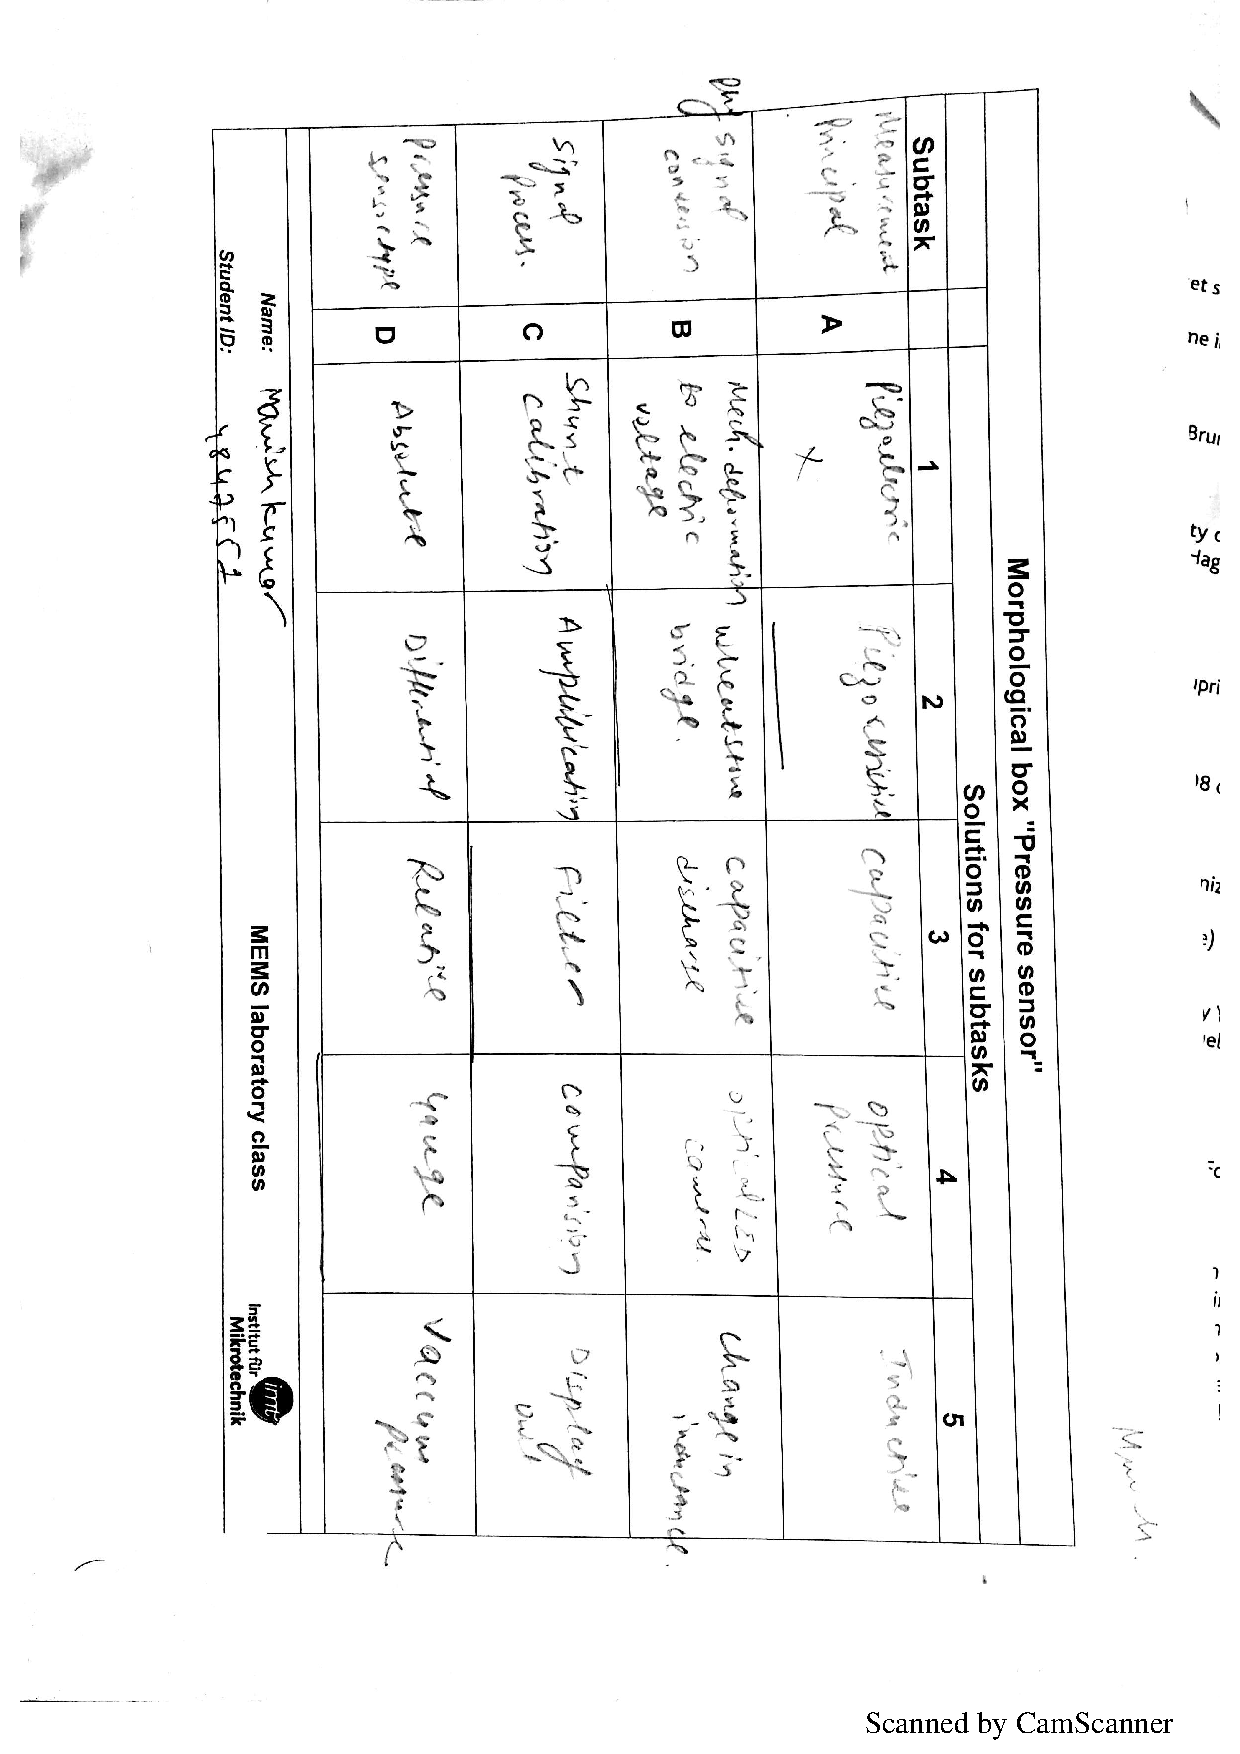
\includepdf[pages={1}, scale=0.7]{figures/Manish.pdf}
\end{figure}
\newpage

\begin{figure}[H]
	\centering
	\includepdf[pages={2}, scale=0.7]{figures/Manish.pdf}
\end{figure}
\newpage

%\begin{figure}[H]
%	\centering
%	\includepdf[pages={3}, scale=0.7]{figures/Manish.pdf}
%\end{figure}
%
%\newpage
%
%\begin{figure}[H]
%	\centering
%	\includepdf[pages={4}, scale=0.7]{figures/Manish.pdf}
%\end{figure}